\documentclass[journal,10pt]{IEEEtran}
\usepackage{graphicx,amsmath,booktabs}
\title{Sizing and Verifying a Two-Stage Differential OTA with Device Lookup Tables}
\author{Fourth design iteration}
\begin{document}
\maketitle
\begin{abstract}
A 180-nm BSIM3 lookup table sets the dimensions of two independently tested stages. The integrated design settles to 0.5\% in 5.62 ns or less at nominal bias. Forty electrical stress conditions and twenty threshold-mismatch samples meet the measured differential settling and phase requirements. The minimum quiescent saturation margin across twelve transistors is 36.66 mV. Nominal power rises from 353.5 to 498.9 $\mu$W relative to iteration three.
\end{abstract}
\section{Design goals and operating point}
The handouts specify a 1.1-V fully differential capacitive-feedback amplifier. The user supplied a 180-nm BSIM3 model for this implementation. The solution report uses the course 45-nm process and reports 75 dB of open-loop gain, about 2 ns of settling and 1.32 mW. Its folded input stage and Hogervorst output illustrate how to distribute gain and source/sink signal current. We use its input/output efficiency targets of 18/15 V$^{-1}$ as starting points. The new design keeps the previous NMOS input pair and uses a direct complementary output path with a separate common-mode sink.
\begin{table}[h]\centering
\caption{Requirements and nominal results at 27$^\circ$C}
\begin{tabular}{lrr}\toprule
Quantity & Requirement & Measured\\\midrule
$C_s/C_f/C_L$ (pF) & 1/.25/.25 & 1/.25/.25\\
Static / dynamic error at 10 ns (\%) & .5 / .5 & .3931 / .0310\\
Dynamic error at 40 ns (\%) & .5 & $<.00004$\\
Differential swing span (V) & .5 & 1.528\\
Output common mode (V) & --- & .5895\\
Input common-mode range (V) & --- & .449--.930\\
Open-loop / loop gain (dB) & --- & 68.74 / 48.18\\
Loop crossover (MHz) & --- & 84.23\\
Differential phase margin (deg) & 60 & 70.42\\
Rise / fall settling, 0.5\% (ns) & 10 / 10 & 5.59 / 5.62\\
CMRR / PSRR (dB) & 60 / 60 & 98.83 / 94.21\\
Input offset sample deviation (mV) & --- & 1.337\\
Output noise ($\mu$V rms) & 600 & 480.8\\
Quiescent power ($\mu$W) & minimize & 498.9\\\bottomrule
\end{tabular}
\end{table}
\section{Single-device characterization}
Following Chapter 5, we simulated a 10-$\mu$m unit device over seven drawn lengths (0.18--0.90 $\mu$m), 12 drain biases (0.08--0.75 V), and 67 gate biases (0.24--0.90 V). NMOS tables include body effect. At each bias we stored $I_D,g_m,g_{ds},V_{DSAT}$ and measured $C_{gg}$ from the imaginary gate current at 1 MHz. Figure~\ref{local} shows two slices at the actual design biases. We select $L$ by the loaded gain and the intrinsic speed estimate $f_T=g_m/(2\pi C_{gg})$, then use $W=I_D/(I_D/W)$. The table contains 61,908 distinct device points including hot slow-NMOS and fast cold-NMOS/PMOS stress data.
\section{Independent stage design}
The single-pole estimate $-\ln(.005)/(2\pi\cdot10\ {\rm ns})$ gives 84.33 MHz. A 25\% design reserve, initial Miller capacitor of 200 fF and estimated feedback factor .125 give $g_{m1}=1.060$ mS. At $g_m/I_D=17$ V$^{-1}$, the required branch current is 62.33 $\mu$A. Iterating the pair's body bias with $V_t=0.75-V_{GS1}$ gives 0.174 V. Through the selected 0.60-$\mu$m NMOS, $I_D/W=1.969$ $\mu$A/$\mu$m. Consequently $W_{1,2}=31.7$ $\mu$m. The load needs 53.4 $\mu$m at the same length. Tail and reference lengths are 0.60 $\mu$m. Their hot slow widths are computed at a common gate voltage of 0.553 V and at different drain voltages. The 25-mV headroom reserve gives widths of 94.8 and 14.1 $\mu$m, respectively.
\begin{figure}[t]\centering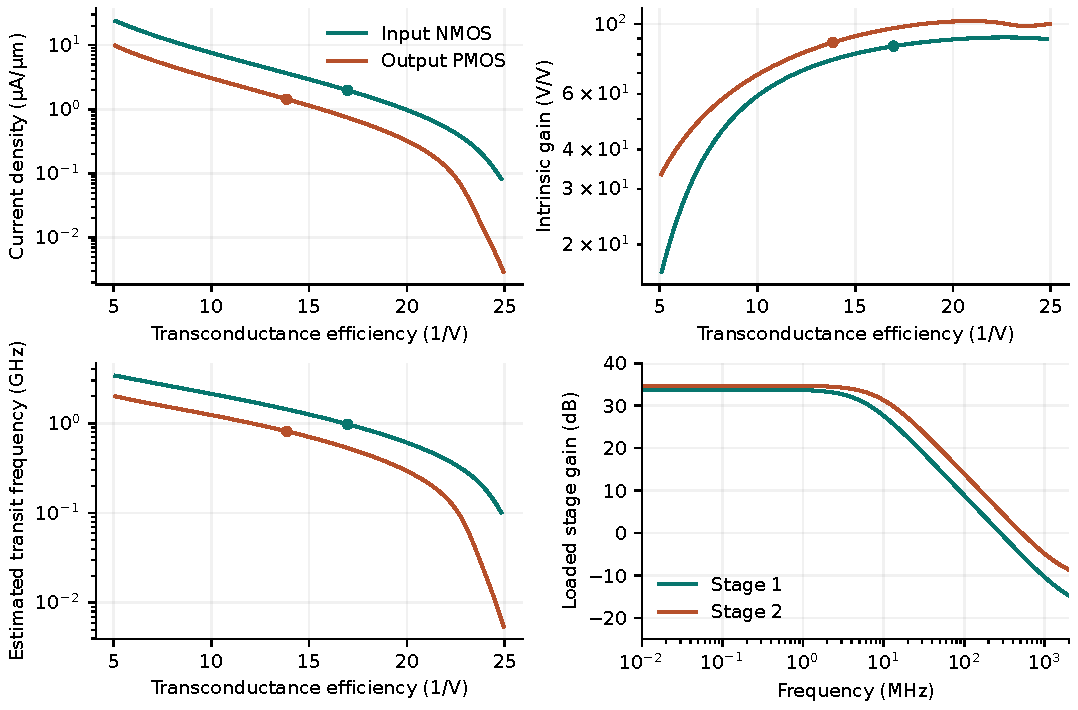
\includegraphics[width=\columnwidth]{sizing}
\caption{Selected NMOS and PMOS operating points on their individual lookup curves. Lower right shows the two independently measured stage responses.}\label{local}
\end{figure}
We allocate gains of 48 and 54 V/V after an initial slow-corner static-error failure. With 450 fF and a conservative 2-M$\Omega$ load per output, the first stage measures 49.05 V/V and a 5.64-MHz bandwidth. Its measured output common mode of 0.51844 V drives the second stage testbench. The final output stage needs 2.265 mS from its complementary paths based on $2\pi(3.8 f_{\rm design})(0.9\ {\rm pF})$. The 0.9 pF is the effective capacitance budget for the internal pole, and the external isolated-stage AC test uses 0.45 pF per side. Fast/cold limits on the NMOS direct-drive share leave at least 60\% of the available pull-up current for the regulated sink at a 0.55-V stress output. At nominal bias the selected share is 4.35\%. This sets $I_{5}=155.3$ $\mu$A by $g_{m2}/[(g_m/I_D)_5+0.0435(g_m/I_D)_9]$. Each device's width follows from its individual current density. The component values are in Fig.~\ref{ckt}. The isolated second stage measures 54.51 V/V and 9.15 MHz.
\begin{figure*}[t]\centering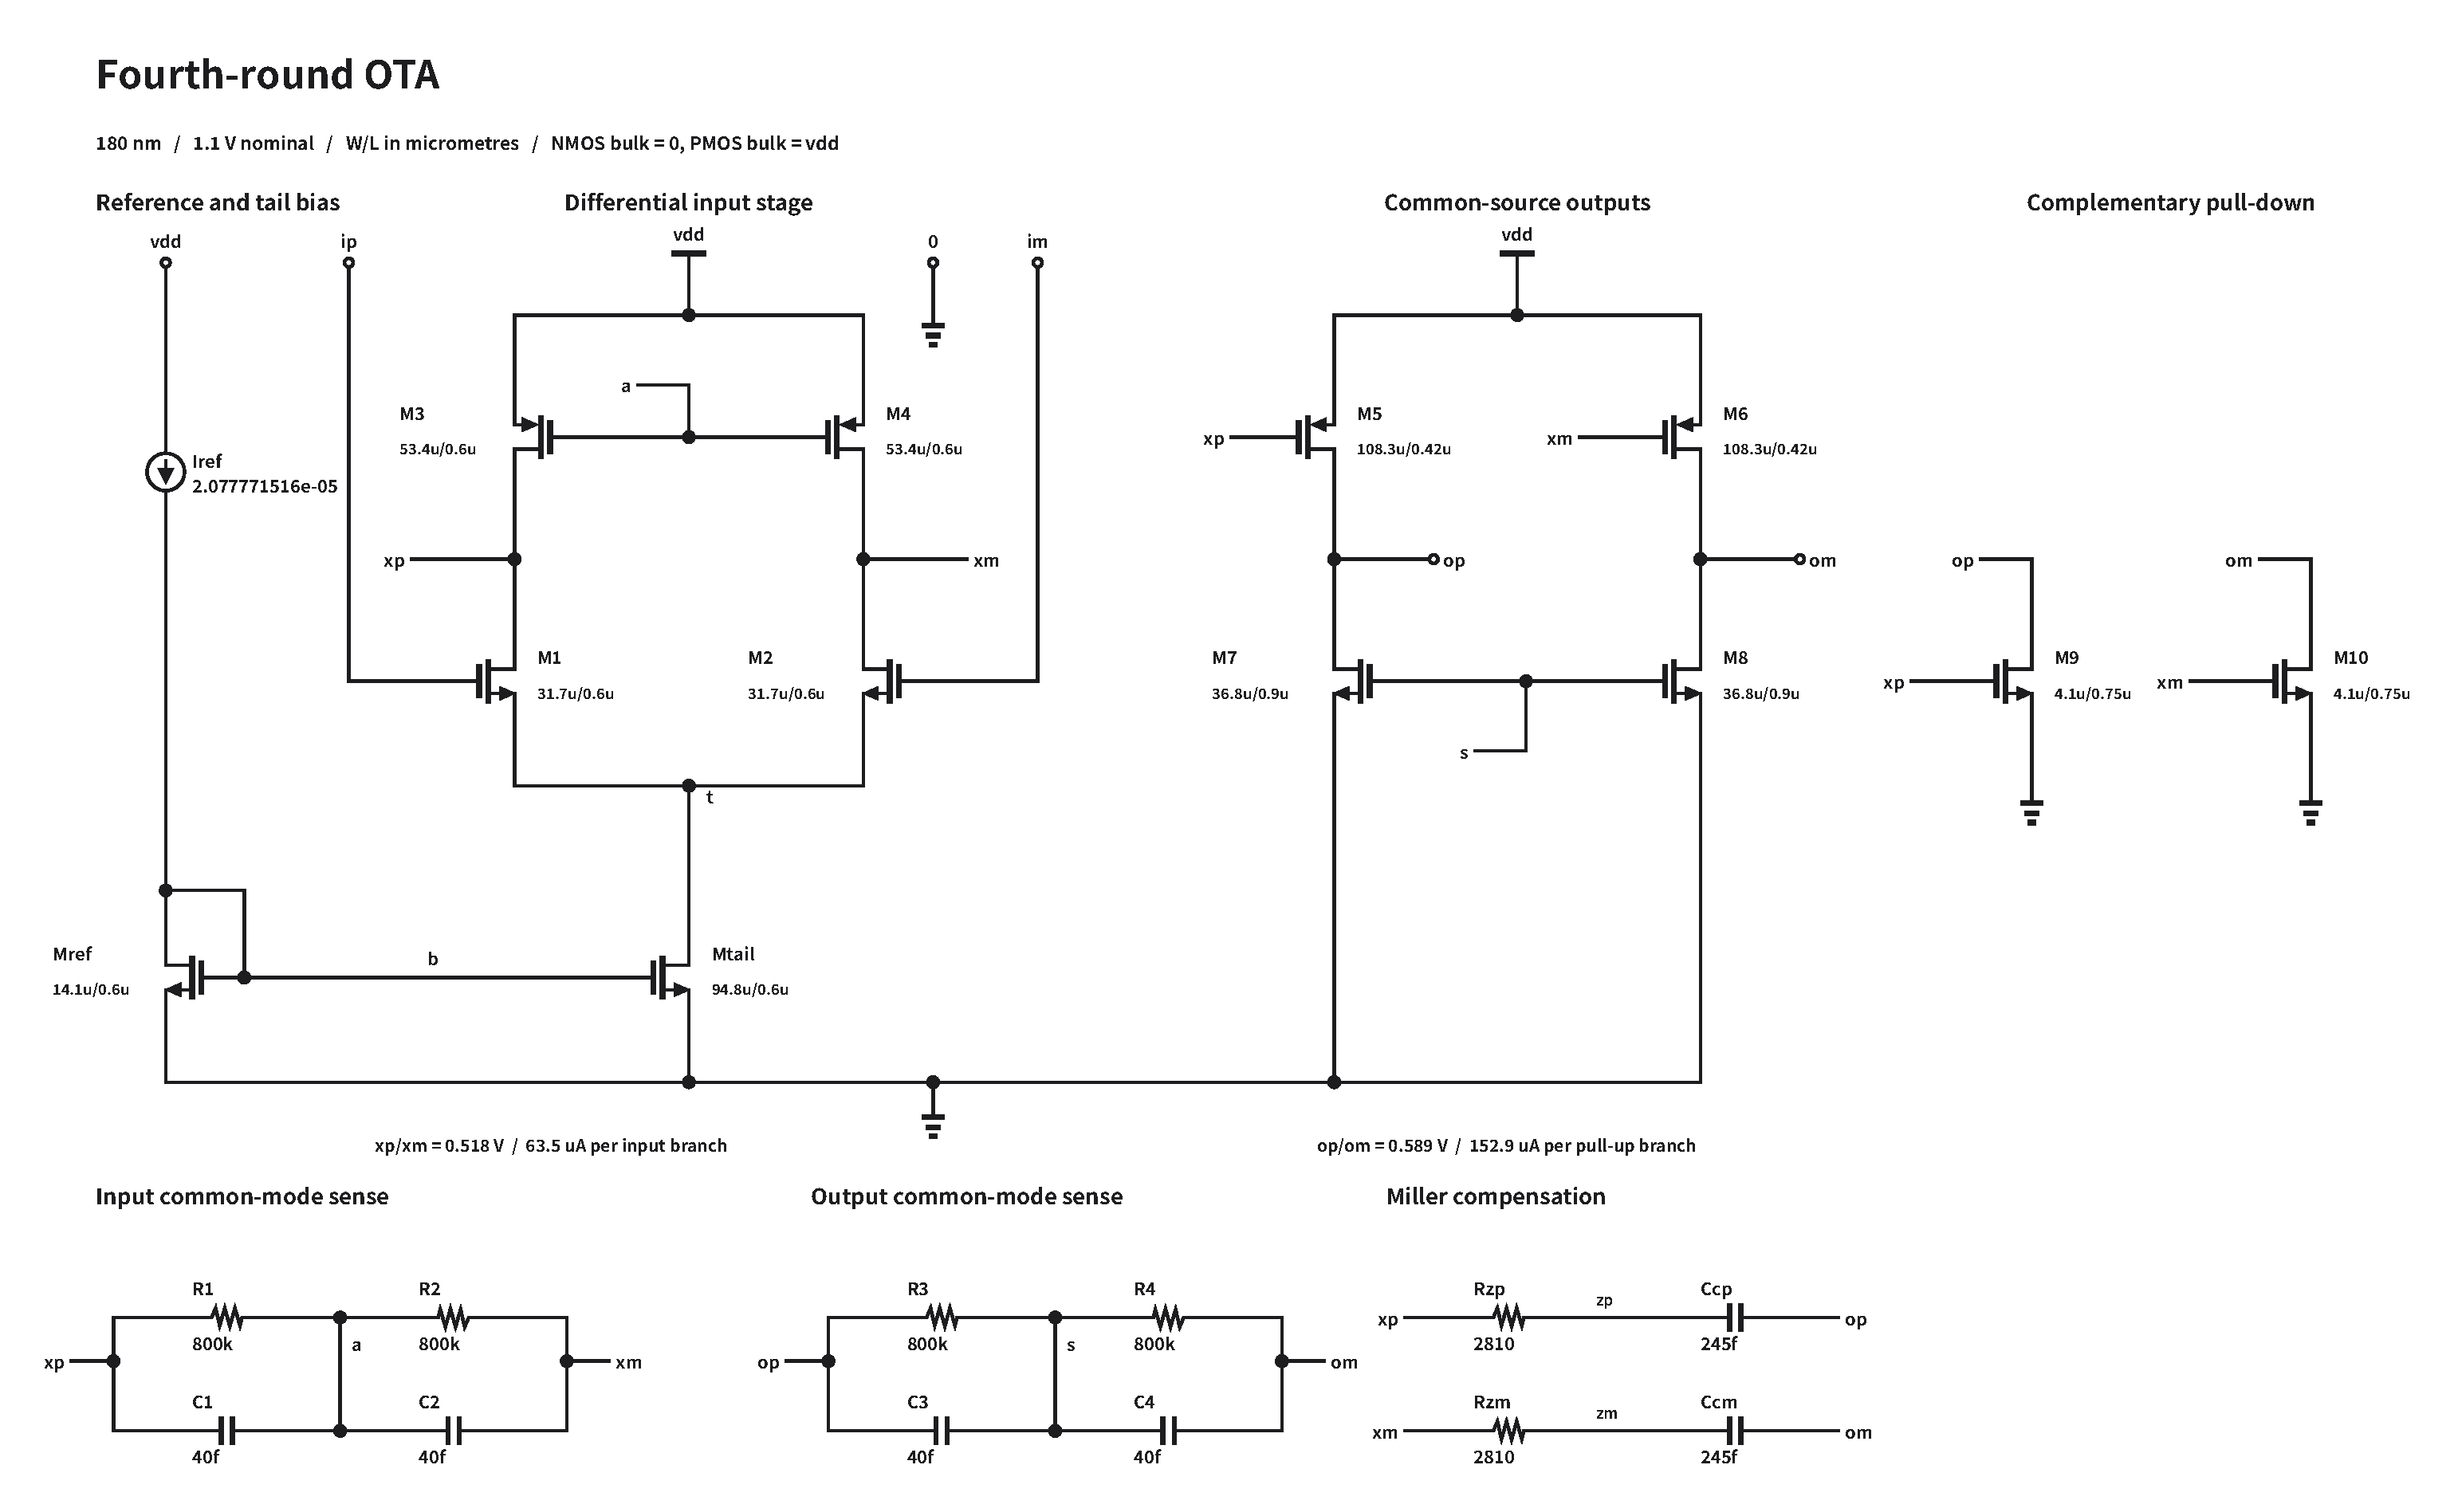
\includegraphics[width=.86\textwidth]{schematic}
\caption{Fourth-round RNL schematic. M9/M10 share the output drain and stage-one gate nets with M5/M6. The separate M7/M8 pair regulates output common mode. Sizes are drawn in micrometres.}\label{ckt}
\end{figure*}
\section{Integration and compensation}
The first resistive gate-drive variant had 50.4 V/V DC gain but a 0.39-MHz local bandwidth and a 15.52-ns rising edge when integrated. Direct drive removed that pole. At 1.2 V fast/cold, the original 25\% standing drive share pulled the integrated output common mode down to 44 mV. A separate fast-device current-density calculation bounded the share using the measured upper input bias of 0.662 V. Raising the output-stage transconductance restored phase margin. With 270 fF, several hot corners still took over 10 ns to settle. We reduced the Miller capacitor to 245 fF and moved its estimated left-half-plane zero to 274 MHz using $R_z=1/g_{m2}+1/(2\pi C_c f_z)=2.81$ k$\Omega$. The measured crossover is 84.23 MHz. A first-order estimate using the realized feedback factor $10^{(48.18-68.74)/20}$, the initial transconductance and 245 fF gives 64.5 MHz. The series zero and the additional poles affect the measured crossover. The product of the two measured local gains gives 68.54 dB, close to 68.74 dB in the complete circuit.
\begin{figure*}[t]\centering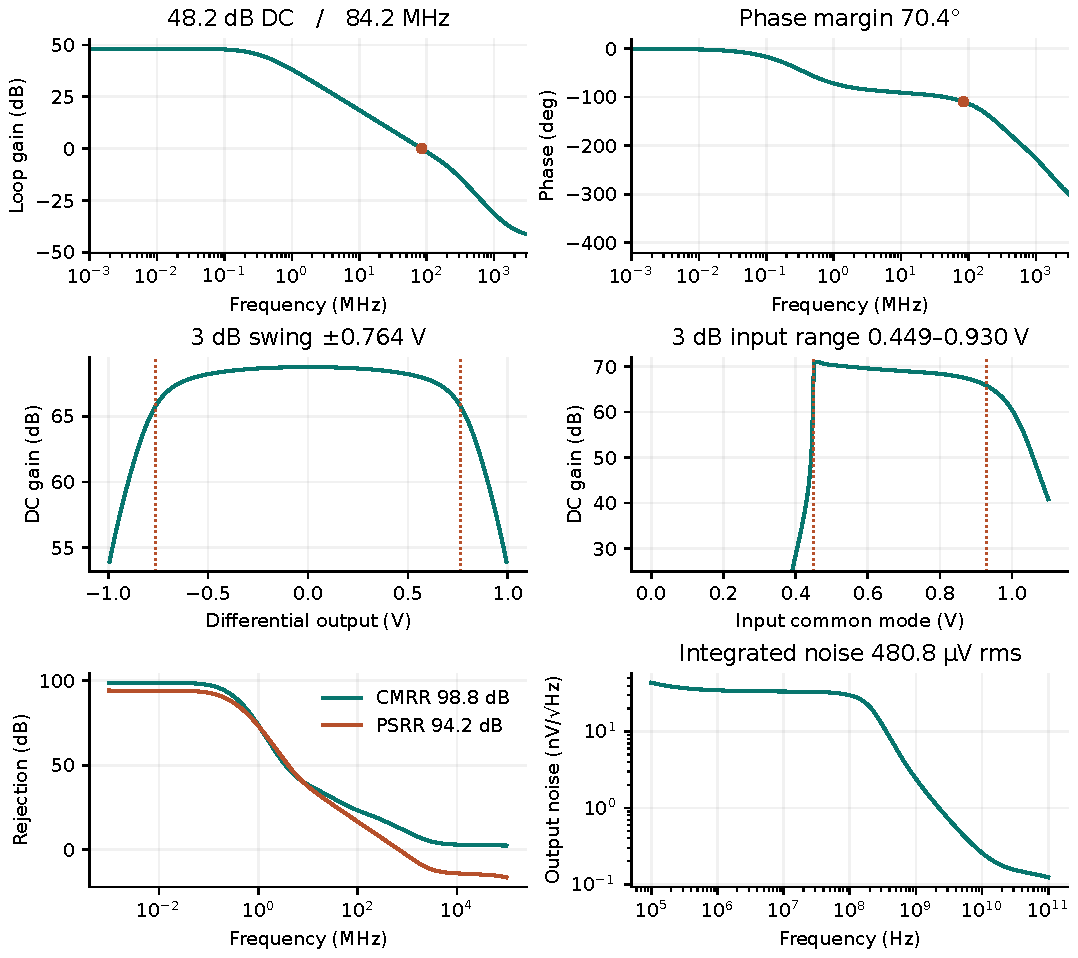
\includegraphics[width=.76\textwidth]{performance}
\caption{Simulated differential loop, swing, common-mode range, rejection and closed-loop output noise. The phase marker is placed at the loop magnitude crossover.}\end{figure*}
\section{Statistical and large-signal verification}
At 1.1 V the reference, input branch pair and output branch pair draw 20.78, 126.97 and 305.77 $\mu$A, respectively. Their power contributions are 22.86, 139.67 and 336.35 $\mu$W. Resistive common-mode sensing carries zero nominal differential DC current. During the specified step the output stage draws 301.1--313.2 $\mu$A from VDD, and the output common mode stays between 0.5888 and 0.5939 V. The two internal common-mode feedback loops have worst phase margins of 72.11 and 75.96 degrees. The external common-mode probe has no unity crossing.
\begin{figure*}[t]\centering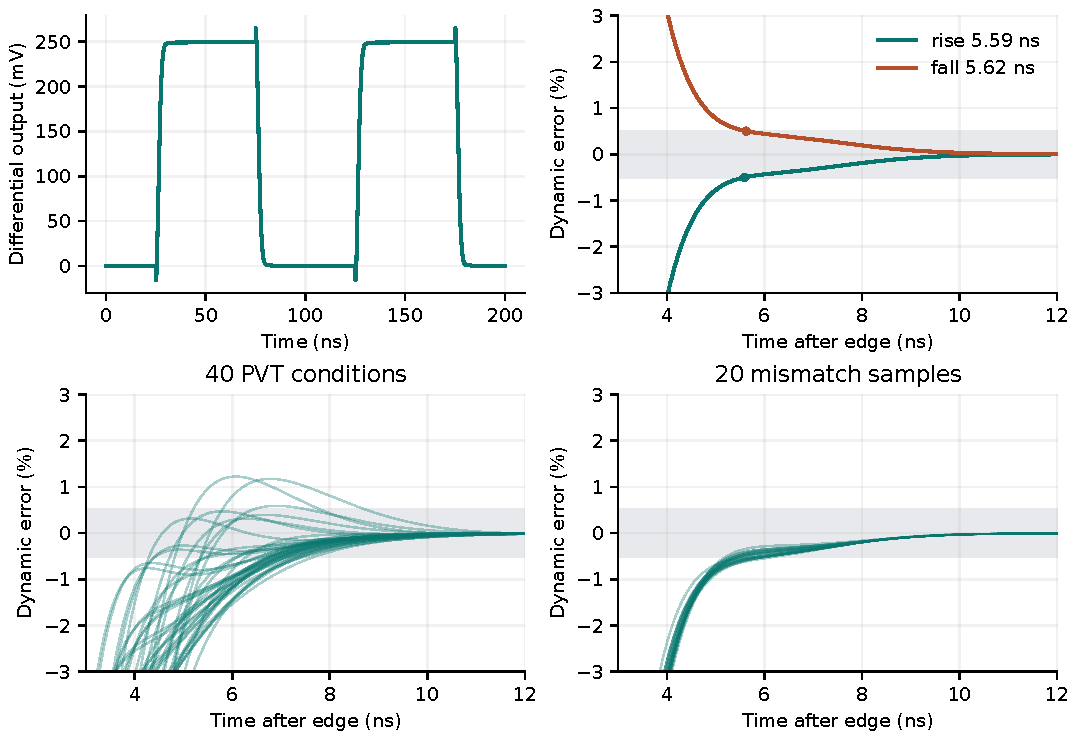
\includegraphics[width=.78\textwidth]{settling}
\caption{Nominal transient, both settling edges and rising edge overlays at all 40 PVT conditions and 20 mismatch seeds. Error is relative to the measured final plateau.}\end{figure*}
\begin{table*}[t]\centering
\caption{Open-loop gain (dB) / loop crossover (MHz) / phase margin (degrees) in each modeled condition}
\begin{tabular}{lrrrrr}\toprule
Corner & Supply (V) & $-25^\circ$C & $-20^\circ$C & $27^\circ$C & $85^\circ$C\\\midrule
TT & 1.1 & 69.6 / 99.2 / 71.5 & 69.5 / 97.6 / 71.4 & 68.7 / 84.2 / 70.4 & 67.7 / 71.4 / 69.4 \\
TT & 1.2 & 70.9 / 101.6 / 73.4 & 70.8 / 99.9 / 73.3 & 70.1 / 86.1 / 72.0 & 69.2 / 72.9 / 70.7 \\
FF & 1.1 & 70.1 / 105.6 / 73.3 & 70.1 / 103.8 / 73.2 & 69.3 / 89.3 / 72.0 & 68.1 / 75.6 / 70.8 \\
FF & 1.2 & 71.4 / 107.9 / 75.1 & 71.3 / 106.1 / 74.9 & 70.6 / 91.1 / 73.5 & 69.6 / 77.1 / 72.1 \\
SS & 1.1 & 69.0 / 92.7 / 69.8 & 69.0 / 91.2 / 69.7 & 68.2 / 78.9 / 69.1 & 67.2 / 66.9 / 68.4 \\
SS & 1.2 & 70.3 / 94.9 / 71.6 & 70.3 / 93.3 / 71.4 & 69.7 / 80.5 / 70.3 & 68.9 / 68.2 / 69.2 \\
FS & 1.1 & 69.3 / 102.1 / 70.0 & 69.2 / 100.4 / 69.9 & 68.3 / 86.5 / 69.0 & 66.9 / 73.3 / 68.1 \\
FS & 1.2 & 70.8 / 105.0 / 72.2 & 70.7 / 103.3 / 72.0 & 70.0 / 88.8 / 70.7 & 69.1 / 75.2 / 69.4 \\
SF & 1.1 & 69.6 / 95.4 / 72.7 & 69.6 / 93.8 / 72.6 & 68.8 / 81.0 / 71.7 & 67.8 / 68.5 / 70.7 \\
SF & 1.2 & 70.8 / 97.4 / 74.4 & 70.7 / 95.7 / 74.3 & 70.1 / 82.5 / 73.1 & 69.2 / 69.7 / 71.8 \\

\end{tabular}
\end{table*}
Input-referred offset has a 1.337-mV sample standard deviation across 20 independent threshold-mismatch realizations. Output noise integrated over 100 kHz--100 GHz is 480.8 $\mu$V rms. Each input NMOS contributes about 230 $\mu$V rms separately. The simulator's per-device noise table is included with the design. Across the 40 PVT conditions the worst dynamic error at 10 ns is 0.162\%, static error 0.464\%, and settling 8.76 ns. Both handout cold temperatures are included. Off-nominal mobilities ($\pm12$\%), thresholds ($\pm25$ mV) and independent threshold mismatch ($3$ mV$\cdot\mu$m$/\sqrt{WL}$) are engineering assumptions. The supplied model contains a nominal pair of cards. Foundry statistical yield and post-layout performance require other data.
\section{Conclusion}
The fourth design trades 145.4 $\mu$W more nominal power and a 0.85-ns slower nominal worst edge for a positive worst-case tail saturation margin, lower integrated noise and shorter worst-case settling across modeled PVT. The saved device sweeps, stage tests and full testbenches allow each of these tradeoffs to be revisited independently.
\end{document}
